

\chapter{Technologies Used}\label{ch:tech}
\bigskip

\section{UDP Cast}

UDP Cast is an open source project that offers a file transfer tool
that can send data simultaneously to many destinations on a \ac{LAN}, under
the \ac{GPL} 2.0 License. The program, along with its source code can be
downloaded from their site, at http://udpcast.linux.lu/.
The compiled projects, offers two executables:  udp-sender and
udp-receiver. By default, the two programs can be used to send input
from standard input on the sever side to all the clients which print
the received data to standard output.

\begin{lstlisting}[caption=Simple udp-sender running]
alexj@lucy:~$ udp-sender
Udp-sender 2004-05-31
Using mcast address 232.168.230.160
UDP sender for (stdin) at 192.168.230.160 on eth0 
Broadcasting control to 192.168.230.255
New connection from 192.168.230.160  (#0) 00000019
Ready. Press any key to start sending data.
Starting transfer: 00000019
Hello
This is a test for the UDP Cast sender & receiver program
bytes= 64 re-xmits=000000 (  0.0%) slice=0162  73 709 551 615 -   0
Transfer complete.
Disconnecting #0 (192.168.230.160)

\end{lstlisting}

\begin{lstlisting}[caption=Simple udp-receiver running]
alexj@lucy:~$ udp-receiver
Udp-receiver 2004-05-31
UDP receiver for (stdout) at 192.168.230.160 on eth0
received message, cap=00000019
Connected as #0 to 192.168.230.160
Listening to multicast on 232.168.230.160
Press any key to start receiving data!
Hello=             64  (  0.71 Mbps) 73 709 551 615 
This is a test for the UDP Cast sender & receiver program
bytes=             64  (  0.00 Mbps) 73 709 551 615 
Transfer complete.
\end{lstlisting}


Using the two simple programs, a file can be transfered to multiple clients
in a single transfer.





\begin{lstlisting}[float,caption=File transfer from a server to two clients]
SERVER:

alexj@hera:~$ cat my_file 
This file has some content.
alexj@hera:~$ udp-sender --file my_file 
Udp-sender 2004-05-31
Using mcast address 232.168.230.160
UDP sender for my_file at 192.168.230.160 on eth0 
Broadcasting control to 192.168.230.255
New connection from 192.168.230.160  (#0) 00000019
Ready. Press any key to start sending data.
New connection from 192.168.230.129  (#1) 00000019
Ready. Press any key to start sending data.
Starting transfer: 00000019
bytes= 28 re-xmits=000000 (  0.0%) slice=0162              28 -   1
Transfer complete.
Disconnecting #0 (192.168.230.160)
Disconnecting #1 (192.168.230.129)

CLIENT 1:

alexj@hera:/tmp$ udp-receiver --file my_local_file
Udp-receiver 2004-05-31
UDP receiver for my_local_file at 192.168.230.160 on eth0
received message, cap=00000019
Connected as #0 to 192.168.230.160
Listening to multicast on 232.168.230.160
Press any key to start receiving data!
bytes= 28  (  0.00 Mbps)             28 
Transfer complete.
alexj@hera:/tmp$ cat my_local_file 
This file has some content.

CLIENT 2:

root@spook:/tmp# udp-receiver --file my_local_file
Udp-receiver 2004-05-31
UDP receiver for my_local_file at 192.168.230.129 on eth0
received message, cap=00000019
Connected as #1 to 192.168.230.160
Listening to multicast on 232.168.230.160
Press any key to start receiving data!
bytes= 28  (  0.00 Mbps)             28 
Transfer complete.
root@spook:/tmp# cat my_local_file 
This file has some content.


\end{lstlisting}


Both programs accept various parameters to change the way in which the
transfer is made. The options include the possibility to send via broadcast
and not multicast, send with a TTL of one (only to the local network) or
send asynchronously (without waiting for an answer from the clients).

\pagebreak
\subsection{udp-sender}
\begin{lstlisting}[caption=Command line flags for udp-sender]

udp-sender [--file file] [--full-duplex] [--half-duplex] [--pipe pipe]
[--portbase portbase] [--blocksize size] [--interface net-interface]
[--mcast-data-address data-mcast-address] [--mcast-rdv-address
mcast-rdv-address] [--max-bitrate bitrate] [--pointopoint] [--async] [--log
file] [--min-slice-size min] [--max-slice-size max] [--slice-size] [--ttl
time-to-live] [--fec stripesxredundancy/stripesize] [--print-seed]
[--rexmit-hello-interval interval] [--autostart autostart] [--broadcast]
[--min-receivers receivers] [--min-wait sec] [--max-wait sec] [--nokbd]
[--retries-until-drop n] [--bw-period n]

\end{lstlisting}



Basic options\cite{man:udp-sender}

--file file

Reads data to be transmitted from file. If this parameter is not
supplied, data to be transmitted is read from stdin instead.

--pipe command

Sends data through pipe before transmitting it. This is useful for
compressing/decompressing it, or for stripping out unused blocks. The
command gets a direct handle on the input file or device, and thus may seek
inside it, if needed. "Udpcast" itself also keeps a handle on the file,
which is used for an informal progress display. The command's stdout is a
pipe to udpcast.

--autostart n

Starts transmission after n retransmissions of hello packet, without
waiting for a key stroke. Useful for unattended operation, where udp-sender
is started from a cron-job for a broadcast/multicast at a scheduled time.

Networking options

The following networking options should be supplied both on the sender and
the receivers:

--portbase portbase

    Default ports to use for udpcast. Two ports are used: portbase and
portbase+1 . Thus, Portbase must be even. Default is 9000. The same
portbase must be specified for both "udp-sender" and "udp-receiver".

--interface interface

    Network interface used to send out the data. Default is "eth0"

--ttl time to live

    Sets the time-to-live parameter for the multicast packets. Should
theoretically allow to use UDPCast beyond the local network, but not tested
for lack of a multicast router.

--mcast-rdv-address address

    Uses a non-standard multicast address for the control (rendez-vous)
connection. This address is used by the sender and receivers to "find" each
other. This is not the address that is used to transfer the actual data.

    By default "mcast-rdv-address" is the Ethernet broadcast address if
"ttl" is 1, and 224.0.0.1 otherwise. This setting should not be used except
in very special situations, such as when 224.0.0.1 cannot be used for
policy reasons.

The following networking options should be supplied only on the sender:

--mcast-data-address address

    Uses the given address for multicasting the data. If not specified, the
program will automatically derive a multicast address from its own IP (by
keeping the last 27 bits of the IP and then prepending 232).

--pointopoint

    Point-to-point mode. Only a single receiver is allowed, but the data
will be directly send to this receiver (in unicast mode), rather than
multicast/broadcast all over the place. If no async mode is chosen, and
there happens to be only one receiver, point-to-point is activated
automatically.

--nopointopoint

    Don't use point-to-point, even if there is only one single receiver.

--full-duplex

    Use this option if you use a full-duplex network. T-base-10 or 100 is
full duplex if equipped with a switch. Hub based networks, or T-base-2
networks (coaxial cable) are only half-duplex and you should not use this
option with these networks, or else you may experience a 10\% performance
hit.

    N.B. On high-latency WAN links, the full-duplex option can lead to
substantial performance improvements, because it allows udp-sender to send
more data while it is still waiting for the previous batch to get
acknowledged.

--half-duplex

    Use half duplex mode (needed for Hub based or T-base-2 networks). This
is the default behavior in this version of udpcast.

--broadcast

    Use Ethernet broadcast, rather than multicast. Useful if you have
Ethernet cards which don't support multicast.

    By default, "udpcast" uses multicast. This allows sending the data only
to those receivers that requested it. Ethernet cards of machines which
don't participate in the transmission automatically block out the packets
at the hardware level. Moreover, network switches are able to selectively
transmit the packets only to those network ports to which receivers are
connected. Both features thus allow a much more efficient operation than
broadcast. This option should only be supplied on the sender.

-b blocksize
    Choses the packet size. Default (and also maximum) is 1456.


Unidirectional mode (without return channel)

The options described below are useful in situations where no "return
channel" is available, or where such a channel is impractical due to high
latency. In an unidirectional setup (i.e. without return channel), the
sender only sends data but doesn't expect any reply from the receiver.

Unidirectional options must be used together, or else the transfer will not
work correctly. You may for example use the following command line:

"udp-sender --async --max-bitrate 10m --fec 8x8"

--async

    Asynchronous mode. Do not request confirmations from the receiver. Best
used together with forward error correction and bandwidth limitation, or
else the receiver will abort the reception as soon as it misses a packet.
When the receiver aborts the reception in such a way, it will print a list
of packets lost in the slice causing the problem. You can use this list to
tune the forward error correction parameters. 

--max-bitrate bitrate

    Limits bandwidth used by udpcast. Useful in asynchronous mode, or else
the sender may send too fast for the switch and/or receiver to keep up.
Bitrate may be expressed in bits per second (--bitrate 5000000), kilobits
per second ("--bitrate 5000k") or megabits per second ("--bitrate 5m").
This is the raw bitrate, including packet headers, forward error
correction, retransmissions, etc. Actual payload bitrate will be lower. 

--fec interleave"x"redundancy"/"stripesize

    Enables forward error correction. The goal of forward error correction
is to transmit redundant data, in order to make up for packets lost in
transit. Indeed, in unidirectional mode, the receivers have no way of
requesting retransmission of lost packets, thus the only way to address
packet loss is to include redundant information to begin with. The
algorithm is designed in such a way that if r redundant packets are
transmitted, that those can be used to compensate for the loss of any r
packets in the same FEC group (stripe).

    In order to increase robustness of the FEC algorithm against burst
packet losses, each slice is divided in interleave stripes. Each stripe has
stripesize blocks (if not specified, stripesize is calculated by diving
slice-size by interleave). For each stripe, redundancy FEC packets are
added. Stripes are organized in such a fashion that consecutive packets
belong to different stripes. This way, we ensure that burst losses affect
different stripes, rather than using all FEC packets of a single stripe.

Example: "--fec 8x8/128" 

--rexmit-hello-interval timeout

    If set, rebroadcasts the HELLO packet used for initiating the casting
each timeout milliseconds.

    This option is useful together with asyc mode, because with async mode
the receiver won't send a connection request to the sender (and hence won't
get a connection reply). In async mode, the receivers get all needed
information from the hello packet instead, and are thus particularly
dependant on the reception of this packet, makeing retransmission useful.

    This option is also useful on networks where packet loss is so high
that even with connection requests, sender and receiver would not find each
other otherwise. 

--retries-until-drop retries

    How many time to send a REQACK until dropping a receiver. Lower
retrycounts make "udp-sender" faster to react to crashed receivers, but
they also increase the probability of false alerts (dropping receivers that
are not actually crashed, but merely slow to respond for whatever reason) 
Keyboardless mode

The options below help to run a sender in unattended mode.

--min-receivers n

    Automatically start as soon as a minimal number of receivers have
connected. 

--min-wait t

    Even when the necessary amount of receivers do have connected, still
wait until t seconds since first receiver connection have passed. 

--max-wait t

    When not enough receivers have connected (but at least one), start
anyways when t seconds since first receiver connection have pased. 

--nokbd

    Do not read start signal from keyboard, and do not display any message
telling the user to press any key to start. 

--daemon-mode

    Do not exit when done, but instead wait for the next batch of
receivers.

Logging options

The options instruct "udp-sender" to log some additional statistics to a
file:

--log file

    Logs some stuff into file. 

--bw-period seconds

    Every so much seconds, log instantenous bandwidth seen during that
period. Note: this is different from the bandwidth displayed to stderr of
the receiver, which is the average since start of transmission. 


\pagebreak
\subsection{udp-receiver}
\begin{lstlisting}[caption= Command line flags for udp-receiver]

udp-receiver [--file file] [--pipe pipe] [--portbase portbase]
[--interface net-interface] [--log file] [--ttl time-to-live]
[--mcast-rdv-address mcast-rdv-address] [--nokbd] [--exitWait milliseconds] 

\end{lstlisting}


Basic options\cite{man:udp-receiver}

--file file

    Writes received data to file. If this parameter is not supplied,
received data is written to stdout instead. 

--pipe command

    Sends data through pipe after receiving it. This is useful for
decompressing the data, or for filling in unused filesystem blocks that may
have been stripped out by udp-sender. The command gets a direct handle on
the output file or device, and thus may seek inside it, if needed.
"Udpcast" itself also keeps a handle on the file, which is used for an
informational progress display. The command's stdin is a pipe from
udp-receiver. Example: "udp-receiver -p "gzip -dc"" 

--log file

    Logs some stuff into file. 

--nosync

    Do not open target in synchronous mode. This is the default when
writing to a file or a pipe. 

--sync

    Write to target in synchronous mode. This is the default when writing
to a device (character or block) 

--nokbd

    Do not read start signal from keyboard, and do not display any message
telling the user to press any key to start. 

--start-timeout sec

    receiver aborts at start if it doesn't see a sender within this many
seconds. Furthermore, the sender needs to start transmission of data within
this delay. Once transmission is started, the timeout no longer applies. 
Networking options

--portbase portbase

    Default ports to use for udpcast. Two ports are used: portbase and
portbase+1 . Thus, Portbase must be even. Default is 9000. The same
portbase must be specified for both "udp-sender" and "udp-receiver". 

--interface interface

    Network interface used to send out the data. Default is "eth0" 

--ttl ttl

    Time to live for connection request packet (by default connection
request is broadcast to the LAN 's broadcast address. If ttl is set, the
connection request is multicast instead to 224.0.0.1 with the given ttl,
which should enable udpcast to work between LANs. Not tested though. 

--mcast-rdv-address address

    Uses a non-standard multicast address for the control connection (which
is used by the sender and receivers to "find" each other). This is not the
address that is used to transfer the data. By default "mcast-rdv-address"
is the Ethernet broadcast address if "ttl" is 1, and 224.0.0.1 otherwise.
This setting should not be used except in very special situations, such as
when 224.0.0.1 cannot be used for policy reasons. 

--exit-wait milliseconds

    When transmission is over, receiver will wait for this time after
receiving the final REQACK . This is done in order to guard against loss of
the final ACK . Is 500 milliseconds by default.


\section{Example of UDP Cast Usage}

On top of the two executables (udp-sender and udp-receiver) the UDP Cast
Project offers a Live CD (that can be found on their website) built to run
a wizard for the configuration for a sender or a receiver of a system
image. The iso file can be burned onto a CD or set up on a PXE network
boot.

The Live CD is a Linux Distribution based on Debian, stripped down to
occupy a small amount of memory and boot very fast. It must be booted on
all workstations that will participate in the imaging process (the seed
that is the sender and all the receivers)

After the kernel loads, it must load kernel modules (device drivers)
for the \ac{NIC} and the hard disk drives.

\begin{figure}[h]
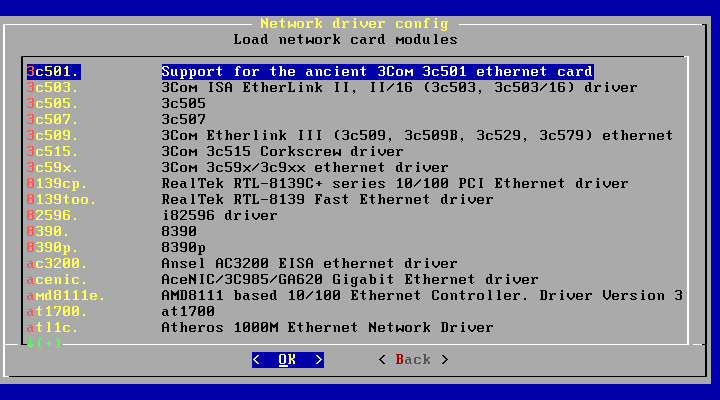
\includegraphics[width=10cm]{img/udpcast_net_module}
\caption{UDP Cast: Selection of the \ac{NIC} Driver}
\label{fig:udpcast_net_module}
\end{figure}



\begin{figure}[h]
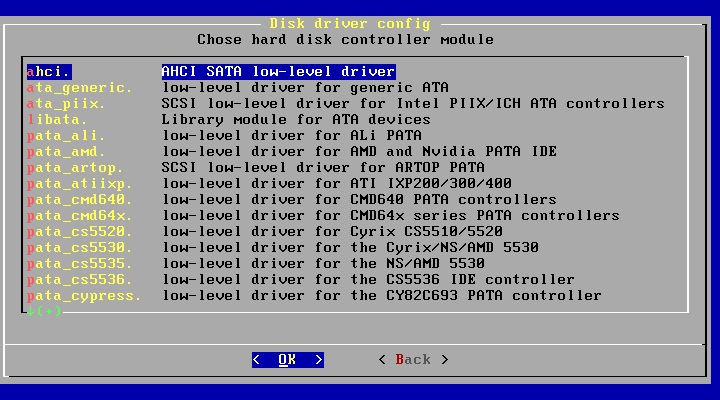
\includegraphics[width=10cm]{img/udpcast_hdd_module}
\caption{UDP Cast: Selection of the \ac{HDD} Driver}
\label{fig:udpcast_hdd_module}
\end{figure}


When the \ac{OS} has loaded the device driver, it can configure
network connectivity. This is done either by setting up a manual IP address
with a valid subnet mask or by use of \ac{DHCP} automatic configuration.
Obtaining an IP address is mandatory for the system to work because,
without an IP, the sender can't connect to the receivers.


\begin{figure}[h]
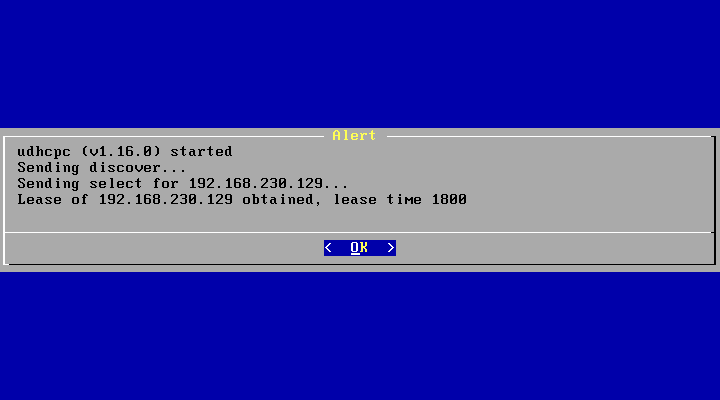
\includegraphics[width=10cm]{img/udpcast_dhcp}
\caption{UDP Cast: Obtaining an IP address via \ac{DHCP}}
\label{fig:udpcast_dhcp}
\end{figure}


After the device driver for the hard disks (PATA, SATA, SCSI) is loaded,
the user must chose what partition or device will be imaged. This has local
significance. On the seed host it will be the partition that will be sent over
the network and on the receivers it will be the partition on which the data
will be written. The name of the partitions are Linux formated. The user
can select a single primary or logical partition (ex. hda1, sda2, sdb5) or
an entire drive (hda, hdb, sda). The \ac{MBR} is found on the first 512bytes of
the physical drive.

It is recommended that the same option be selected on all devices.

\begin{figure}[h]
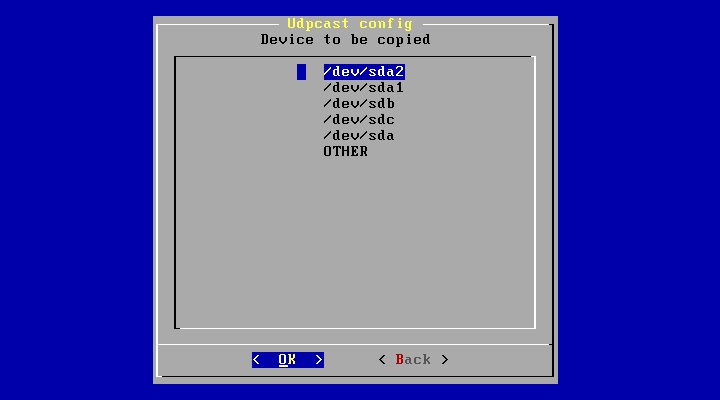
\includegraphics[width=10cm]{img/udpcast_partitions}
\caption{UDP Cast: Selection of the imaged device(physical driver or
partition}
\label{fig:udpcast_partitions}
\end{figure}


A partition is usually has a very large data size and the transfer over the
network could be time consuming. For computers with good enough processing
power, compression can be used. UDP Cast offers two types of compression
\begin{itemize}
\item \ac{LZOP}
\item \ac{GZIP}
\end{itemize}

The use of compression can reduce the sent data by a factor of up to 50\%.

\begin{figure}[h]
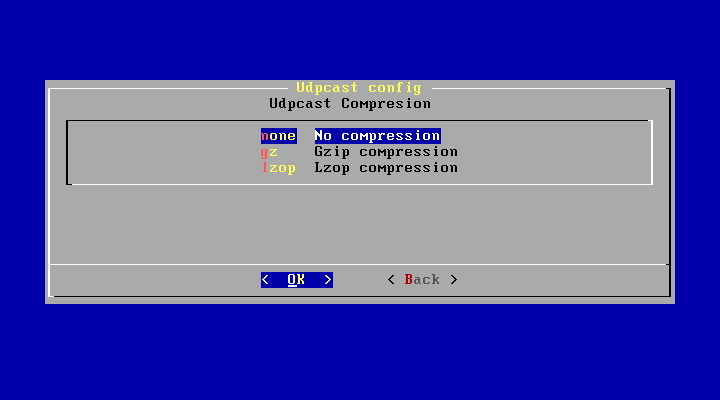
\includegraphics[width=10cm]{img/udpcast_compression}
\caption{UDP Cast: Selection of compression algorithm.}
\label{fig:udpcast_compression}
\end{figure}

After all the configurations are made (they should be identical in most
conditions), the direction of the transfer must be specified on each host.
One workstation will be the sender and all the others will be the
receivers.

\begin{figure}[h]
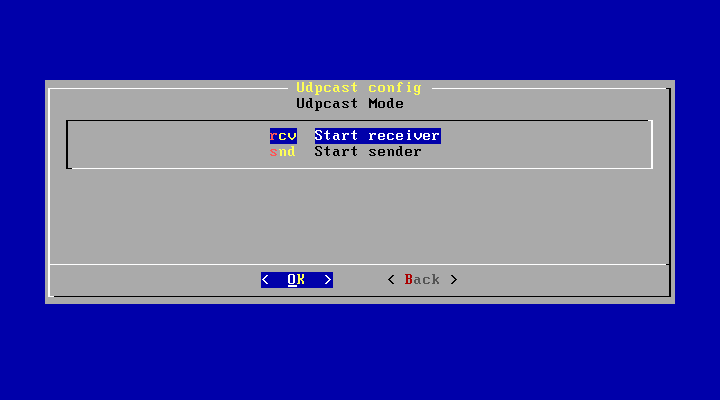
\includegraphics[width=10cm]{img/udpcast_mode}
\caption{UDP Cast: Selection of sender or receiver mode.}
\label{fig:udpcast_mode}
\end{figure}



\section{Multicast}

In the classic client-server model, each connection between a client and
the server is a separate data stream. This means, that if a server has 1000
clients, it needs to open 1000 connections each with it's stream of data.
This is normal, because each connection sends unique data.

But in the case of live streaming (such as audio or video stream) one
server sends the same information to all of it's clients, and using the
classic model, this would mean redundant copied information across the
network. Multicast comes in these kinds of situations and it optimises
the traffic by assuring that the server sends only one data stream and that
data stream is delivered to all of the clients that requested the data.

The imaging data sent during an UDP Cast transfer has the same
characteristics as audios and video streaming so it can be considered live
data, making the use of multicast in the transfer the ideal choice. Unicast
would not scale for the server because if it has more connections it has to
cycle through them all to send something and broadcast would send unwanted
traffic to stations that don't participate in the imaging process.

\subsection{Basics of Multicast}

\cite{cisco:multicast}
\ac{IP} multicast is a bandwidth-conserving technology that
reduces traffic by simultaneously delivering a single stream of information
to thousands of corporate recipients and homes. Applications that take
advantage of multicast include videoconferencing, corporate communications,
distance learning, and distribution of software, stock quotes, and news.

IP Multicast delivers source traffic to multiple receivers without adding
any additional burden on the source or the receivers while using the least
network bandwidth of any competing technology. Multicast packets are
replicated in the network by routers enabled with
\ac{PIM} and other supporting multicast protocols
resulting in the most efficient delivery of data to multiple receivers
possible. All alternatives require the source to send more than one copy of
the data. Some even require the source to send an individual copy to each
receiver. If there are thousands of receivers, even low-bandwidth
applications benefit from using IP Multicast. High-bandwidth
applications, such as MPEG video, may require a large portion of the
available network bandwidth for a single stream. In these applications, the
only way to send to more than one receiver simultaneously is by using IP
Multicast.


\begin{figure}[h]
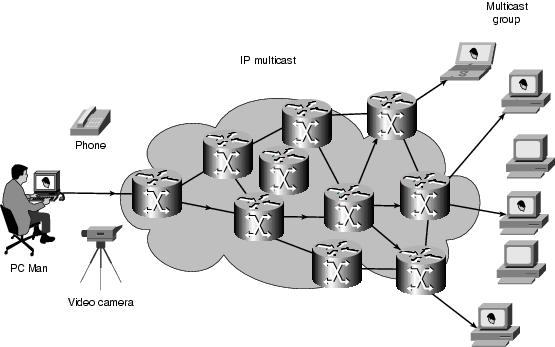
\includegraphics[width=10cm]{img/multicast}
\caption{Multicast Transmission Sending a Single Multicast Packet Addressed
to All Intended Recipients}
\label{fig:multicast}
\end{figure}

\subsection{Multicast Group Concept}

\cite{cisco:multicast}
Multicast is based on the concept of a group. An arbitrary group of
receivers expresses an interest in receiving a particular data stream. This
group does not have any physical or geographical boundaries—the hosts can
be located anywhere on the Internet. Hosts that are interested in receiving
data flowing to a particular group must join the group using \ac{IGMP}.
Hosts must be a member of the group to receive the data stream.


\subsection{IP Multicast Addresses}

\cite{cisco:multicast}
Multicast addresses specify an arbitrary group of IP hosts that have joined
the group and want to receive traffic sent to this group.

The \ac{IANA}  controls the assignment of
IP multicast addresses. It has assigned the old Class D address space to be
used for IP multicast. This means that all IP multicast group addresses
will fall in the range of 224.0.0.0 to 239.255.255.255. 

The \ac{IANA} has reserved addresses in the 224.0.0.0 through 224.0.0.255
to be
used by network protocols on a local network segment. Packets with these
addresses should never be forwarded by a router; they remain local on a
particular LAN segment. They are always transmitted with a time-to-live
(\ac{TTL}) of 1.

\subsubsection{Reserved Link Local Addresses}

\cite{cisco:multicast}
Network protocols use these addresses for automatic router discovery and to
communicate important routing information. For example, OSPF uses 224.0.0.5
and 224.0.0.6 to exchange link state information. 

\begin{table}


\begin{tabular}{| l | r |}
\hline
224.0.0.1 & All systems on this subnet \\
\hline
224.0.0.2 & All routers on this subnet \\
\hline
224.0.0.5 & OSPF routers \\
\hline
224.0.0.6 & OSPF designated routers \\
\hline
224.0.0.12 & DHCP server/relay agent \\
\hline
\end{tabular}
\caption{Multicast Link Local Addresses}
\label{table:multicast_addressed}
\end{table}

\subsubsection{Globally Scoped Address}
\cite{cisco:multicast}
The range of addresses from 224.0.1.0 through 238.255.255.255 are called
globally scoped addresses. They can be used to multicast data between
organizations and across the Internet.

Some of these addresses have been reserved for use by multicast
applications through \ac{IANA}. For example, 224.0.1.1 has been reserved for
\ac{NTP}.

More information about reserved multicast addresses can be found at
http://www.isi.edu/in-notes/iana/assignments/multicast-addresses.


\subsubsection{Limited Scope Addresses}


\cite{cisco:multicast}
The range of addresses from 239.0.0.0 through 239.255.255.255 contains
limited scope addresses or administratively scoped addresses. These are
defined by RFC 2365 to be constrained to a local group or organization.
Routers are typically configured with filters to prevent multicast traffic
in this address range from flowing outside an \ac{AS} or any
user-defined domain. Within an autonomous system or domain, the limited
scope address range can be further subdivided so those local multicast
boundaries can be defined. This also allows for address reuse among these
smaller domains.

\subsubsection{Glop Addressing}
\cite{cisco:multicast}

RFC 2770 proposes that the 233.0.0.0/8 address range be reserved for
statically defined addresses by organizations that already have an AS
number reserved. The AS number of the domain is embedded into the second
and third octets of the 233.0.0.0/8 range.

For example, the AS 62010 is written in hex as F23A. Separating out the two
octets F2 and 3A, we get 242 and 58 in decimal. This would give us a subnet
of 233.242.58.0 that would be globally reserved for AS 62010 to use. 

\subsubsection{Layer 2 Multicast Addresses}

\cite{cisco:multicast}
Normally, \ac{NIC} on a \ac{LAN} segment will receive only
packets destined for their burned-in MAC address or the broadcast MAC
address. Some means had to be devised so that multiple hosts could receive
the same packet and still be capable of differentiating among multicast
groups.

Fortunately, the IEEE \ac{LAN} specifications made provisions for the
transmission of broadcast and/or multicast packets. In the 802.3 standard,
bit 0 of the first octet is used to indicate a broadcast and/or multicast
frame.

\subsubsection{Ethernet MAC Address Mapping}

\cite{cisco:multicast}
The \ac{IANA} owns a block of Ethernet MAC addresses that start with 01:00:5E in
hexadecimal. Half of this block is allocated for multicast addresses. This
creates the range of available Ethernet MAC addresses to be 0100.5e00.0000
through 0100.5e7f.ffff.

This allocation allows for 23 bits in the Ethernet address to correspond to
the IP multicast group address. The mapping places the lower 23 bits of the
IP multicast group address into these available 23 bits in the Ethernet
address.

\subsubsection{Internet Group Management Protocol}

\cite{cisco:multicast}
\ac{IGMP} is used to dynamically register individual hosts in a multicast group
on a particular \ac{LAN}. Hosts identify group memberships by sending
\ac{IGMP}
messages to their local multicast router. Under \ac{IGMP}, routers listen to
\ac{IGMP} messages and periodically send out queries to discover which groups
are active or inactive on a particular subnet.


\subsubsection{Multicast Forwarding}

\cite{cisco:multicast}
In unicast routing, traffic is routed through the network along a single
path from the source to the destination host. A unicast router does not
really care about the source address—it only cares about the destination
address and how to forward the traffic towards that destination. The router
scans through its routing table and then forwards a single copy of the
unicast packet out the correct interface in the direction of the
destination.

In multicast routing, the source is sending traffic to an arbitrary group
of hosts represented by a multicast group address. The multicast router
must determine which direction is upstream (toward the source) and which
direction (or directions) is downstream. If there are multiple downstream
paths, the router replicates the packet and forwards the traffic down the
appropriate downstream paths—which is not necessarily all paths. This
concept of forwarding multicast traffic away from the source, rather than
to the receiver, is called reverse path forwarding. 

\subsubsection{Reverse Path Forwarding}

\cite{cisco:multicast}
\ac{RPF} is a fundamental concept in multicast routing
that enables routers to correctly forward multicast traffic down the
distribution tree. \ac{RPF} makes use of the existing unicast routing table to
determine the upstream and downstream neighbors. A router forwards a
multicast packet only if it is received on the upstream interface. This
\ac{RPF}
check helps to guarantee that the distribution tree will be loop-free. 

\section{UDP over Multicast}

\ac{UDP} is a Transport Layer Protocol in the TCP/IP Stack. The other
protocol at this layer is \ac{TCP}.

The two protocols, TCP and UDP both assure the correct transmission of the
data from a sender process to a receiver process, but the difference is
that TCP is a Reliable Transfer Protocol, while UDP is Best Effort. This
means that TCP guaranties that the data is sent to the destination while
UDP sends the data and hopes it gets safely.

Although TCP is reliable, the transmission of data using TCP has overhead
both in size of the data(larger headers) and in time (TCP needs to have
packets acknowledged). Hence UDP has bigger transmission speeds.

In real lime data streaming (like video, audio streaming), the reliability
of the transmission is not as important as the speed of sending the data.
This makes UDP the normal choice for live data streaming.

Because of how IP Multicast works, UDP is the Transport Layer Protocol of
choice. The sender doesn't need to have the clients acknowledge what it
sends, so reliability is not important. Speed is, because everything has to
real lime.

In UDP Cast, UDP over Multicast is used because of it's speed. This means
that if packets are dropped, at the Transport Layer, they are ignored. But
in an Imaging System, it is not acceptable to have packets ignored because
the packets can be pieces of files. A reliability mechanism has to be in
place, at the Application Layer to ensure that all the data is sent
correctly.

UPC Cast uses ACKs at the Application Layer and a system of timers that
timeout dropped packets so they can be resent.


\section{PXE}


PXE (Preboot eXecution Environment or Pre-Execution
Environment)\cite{wiki:pxe} is a
framework that allows the loading of an Operating System over the network
without having to have any disks on the workstation. It is dependent on
other protocols and concepts such as \ac{IP}, \ac{UDP}, \ac{DHCP} and
\ac{TFTP}.

To boot a system image through \ac{PXE}, you first need to have a workstation
that supports \ac{PXE} in hardware. The Motherboard of the PC must have this
feature and the \ac{BIOS} mush offer the user the option for network boot.

After the chose the network boot, it loads the \ac{PXE} Loader from a ROM on the
Mainboard. This Loader needs to support the whole TCP/IP stack and be able
to start a \ac{DHCP} Client.

The \ac{DHCP} Clients requests an IP address for network connectivity.
For \ac{PXE}
to work, you need to have a server (usually the \ac{DHCP} server) that has a
\ac{TFTP} server that can serve system images. The \ac{DHCP} server passes to the
client along with the IP address and the subnet mask an option (option 200)
for a \ac{TFTP} server.

When the \ac{PXE} enabled client has network connectivity, it can contact the
\ac{TFTP} server and request a system image. The image is downloaded and loaded
into the physical memory of the workstation like a normal \ac{OS}.
